\documentclass [a4paper] {article}
\usepackage[utf8]{inputenc}
\title{Ciencia de datos, práctica 2}
\author{Juan Casado Ballesteros, Samuel García Gonzalez, Iván Anaya Martín}
\usepackage{Sweave}
\begin{document}
\maketitle

\begin{abstract}

\end{abstract}

\newpage
\tableofcontents
\newpage


\section{EJ1}

\section{EJ2}
Creamos un .txt con los datos proporcionados sobre el radio y densidad de los planetas y lo leemos.
\begin{Schunk}
\begin{Sinput}
> datos2 <- read.table("datos2.txt")
> datos2
\end{Sinput}
\begin{Soutput}
    Nombre Radio Densidad
1 Mercurio   2.4      5.4
2    Venus   6.1      5.2
3   Tierra   6.4      5.5
4    Marte   3.4      3.9
\end{Soutput}
\end{Schunk}

Calculamos la regresión sobre dichos datos para obtener la recta que más se aproxime a los puntos que tenemos.
\begin{Schunk}
\begin{Sinput}
> regresion2 <- lm(Densidad~Radio, data=datos2)
> regresion2_own <- regLine(datos2$Radio, datos2$Densidad)
\end{Sinput}
\end{Schunk}

Podemos ver los valores que adopta la ecucaión de la recta que se generará.

y = ax + b

b=
\begin{Schunk}
\begin{Sinput}
> regresion2$coefficients[1]
\end{Sinput}
\begin{Soutput}
(Intercept) 
   4.362396 
\end{Soutput}
\begin{Sinput}
> regresion2_own$coefficients[1]
\end{Sinput}
\begin{Soutput}
[1] 4.362396
\end{Soutput}
\end{Schunk}

a=
\begin{Schunk}
\begin{Sinput}
> regresion2$coefficients[2]
\end{Sinput}
\begin{Soutput}
    Radio 
0.1393669 
\end{Soutput}
\begin{Sinput}
> regresion2_own$coefficients[2]
\end{Sinput}
\begin{Soutput}
[1] 0.1393669
\end{Soutput}
\end{Schunk}

Cuando calculamos la recta de regresión sobre unos datos es necesario evaluar la calidad de esta.
Debemos analizar cómo de bien se ajusta a nuestros datos.
Podemos ver esta información mediante summary.

\subsection{Residuos}
Diferencias entre cada valor de y real y cada valor de y obtenido mediante la función de regresión.
\begin{Schunk}
\begin{Sinput}
> summary(regresion2)$residuals
\end{Sinput}
\begin{Soutput}
          1           2           3           4 
 0.70312301 -0.01253452  0.24565541 -0.93624389 
\end{Soutput}
\end{Schunk}

\subsection{Coeficientes}
Coeficientes estimados para y error estándar para cada uno de ellos.
\begin{Schunk}
\begin{Sinput}
> summary(regresion2)$coefficients
\end{Sinput}
\begin{Soutput}
             Estimate Std. Error   t value   Pr(>|t|)
(Intercept) 4.3623964  1.2049754 3.6203201 0.06854492
Radio       0.1393669  0.2466205 0.5651067 0.62893696
\end{Soutput}
\end{Schunk}

\subsection{Error estándar}
Podemos comprobar que coincide con nuestra implementación.
Cuanto más próximo a 0 sea el error estándar mejor será la recta de regresión.
\begin{Schunk}
\begin{Sinput}
> summary(regresion2)$sigma
\end{Sinput}
\begin{Soutput}
[1] 0.8460019
\end{Soutput}
\begin{Sinput}
> errorEstandar(datos2$Radio, datos2$Densidad, regresion2)
\end{Sinput}
\begin{Soutput}
    Radio 
0.8460019 
\end{Soutput}
\end{Schunk}

\subsection{Correlación cuadrada}
Podemos comprobar que coincide con nuestra implementación.
Este valor está entre 0 y 1 siendo mejor cuanto más próximo a 1 sea (idealmente a partir de 0.8).
\begin{Schunk}
\begin{Sinput}
> summary(regresion2)$r.squared
\end{Sinput}
\begin{Soutput}
[1] 0.1376878
\end{Soutput}
\begin{Sinput}
> correlacionCuadrada(datos2$Radio, datos2$Densidad)
\end{Sinput}
\begin{Soutput}
    Radio 
0.1376878 
\end{Soutput}
\end{Schunk}

Para finalizar dibujaremos una gráfica en la que se representarán lod datos junto a la recta de regresión.
Paralela a la recta de regresión dibujaremos las rectas que marcan el error estándar entorno a la recta de regresión.
En trazado gris grueso la que marca la región en la que estarán el 66\% de los datos y en gris fino la que marca el 95\%.

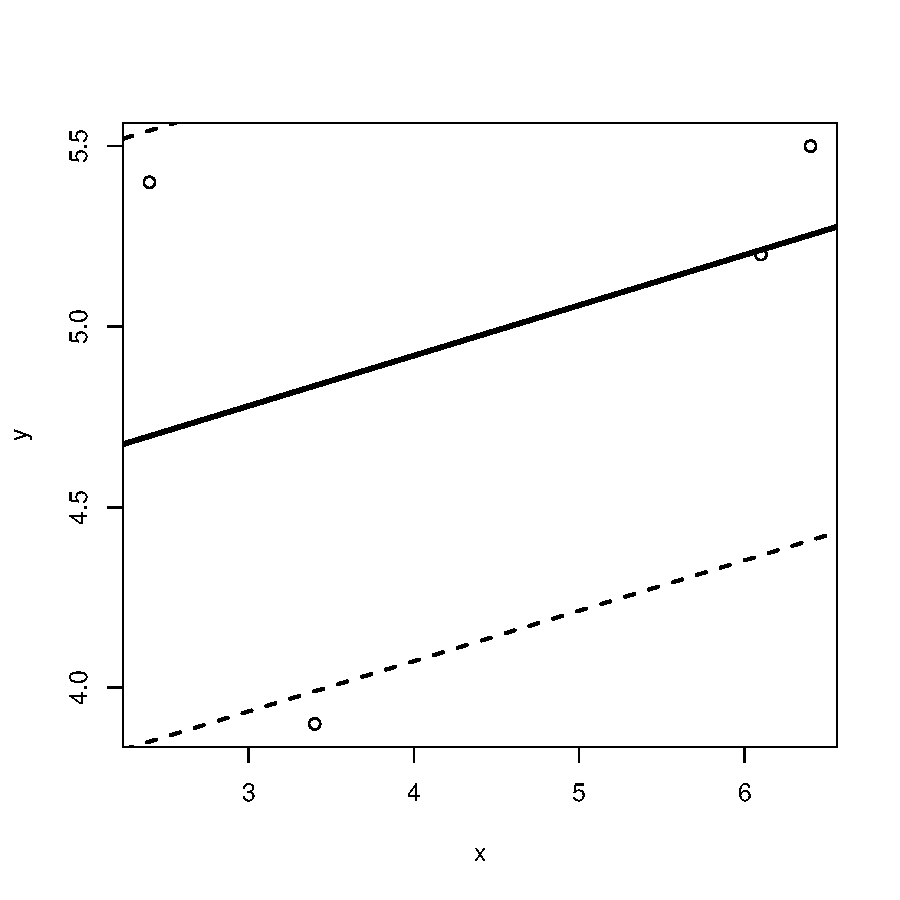
\includegraphics{entrega2-plot_regresion2}

Como podemos ver la recta se ajusta muy mal a los datos que tenemos quedando las rectas que marcan el error estandas fuera del gráfico.
La correlación cuadrada obtenida es muy baja.
En parte esto se debe a que tenemos muy pocos datos.


\section{EJ3}

En esta parte realizamos el algoritmo Hunt con la librería rpart sobre los datos de los vehículos.
Lo primero sera realizar el ejercicio usando Gini como metodo para calculart la impureza.
La segunda parte la calcularemos usando la entropia. 
Por último utilizaremos la libreria tree para repetir estos cálculos aunque solo podremos utilizar Gini para calcular la impuraza.
En ambos casos mostraremos los árboles obtenidos con las librerías adecuadas.

\begin{center}
\begin{Schunk}
\begin{Sinput}
> muestra3 = data.frame(read.table("datos3.txt"))
> clas_3gini=rpart(TipoVehiculo~., data=muestra3,method="class",minsplit=1)
> rpart.plot(clas_3gini)
\end{Sinput}
\end{Schunk}
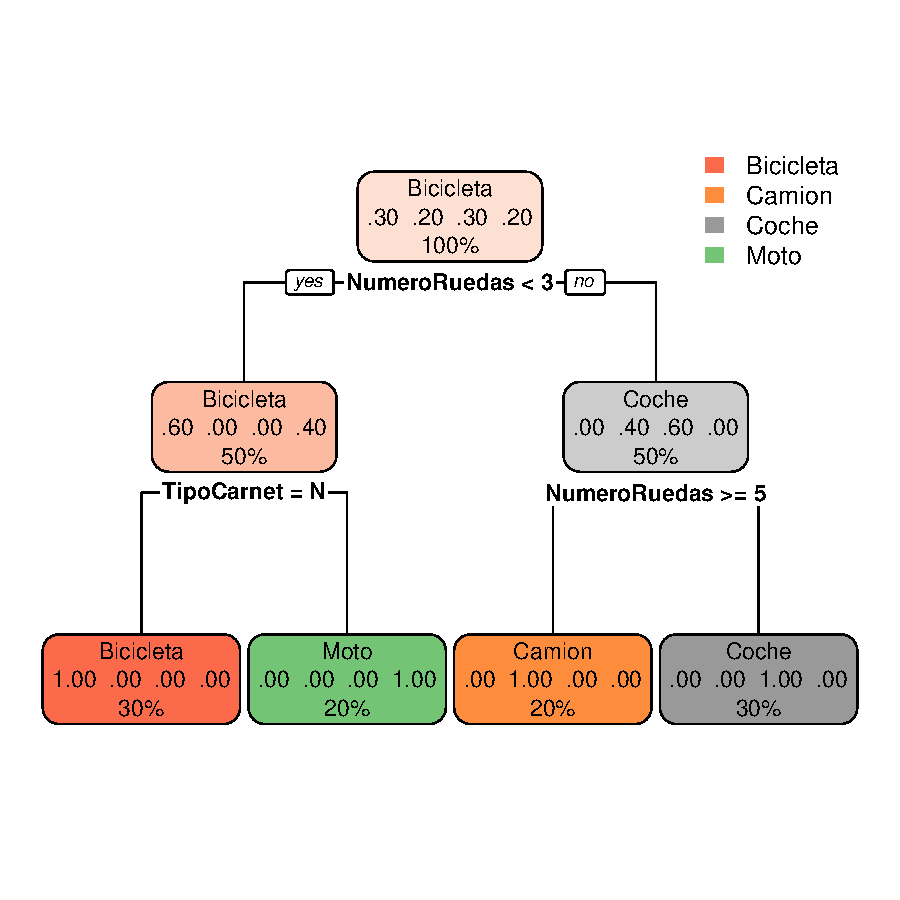
\includegraphics{entrega2-rpart_gini}
\end{center}

Ahora utilizaemos la entropia. 
Para ello añadimos el parametro parms=list(split="information").
Por defecto esta se clasifica por Gini.

\begin{center}
\begin{Schunk}
\begin{Sinput}
> clas_3entropia=rpart(TipoVehiculo~., data=muestra3,method="class",minsplit=1,parms=list(split="information"))
> rpart.plot(clas_3entropia)
\end{Sinput}
\end{Schunk}
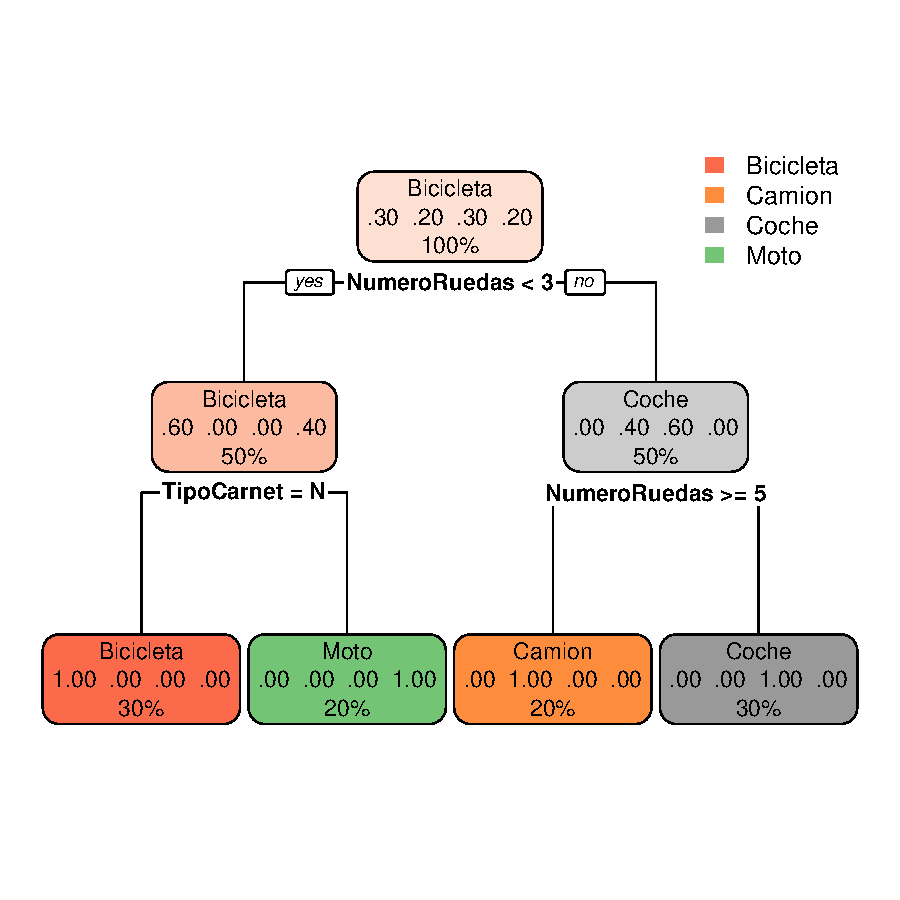
\includegraphics{entrega2-rpart_gini}
\end{center}

Vemos que el árbol obtenido es distinto.
La primera diferencia que se observa, en el caso del arbol Gini su profundidad es de 3 mientras que con Entropia es de 2. 
Es preferible por tanto la clasificación utilizando entropia pues el tiempo de búsqueda en el árbol será menor.

Ahora realizamremos los mismo cálculos con tree.

\begin{center}
\begin{Schunk}
\begin{Sinput}
> clas_3tree=tree(TipoVehiculo~.,data=muestra3,mincut=1,minsize=2) 
> draw.tree(clas_3tree)
\end{Sinput}
\end{Schunk}
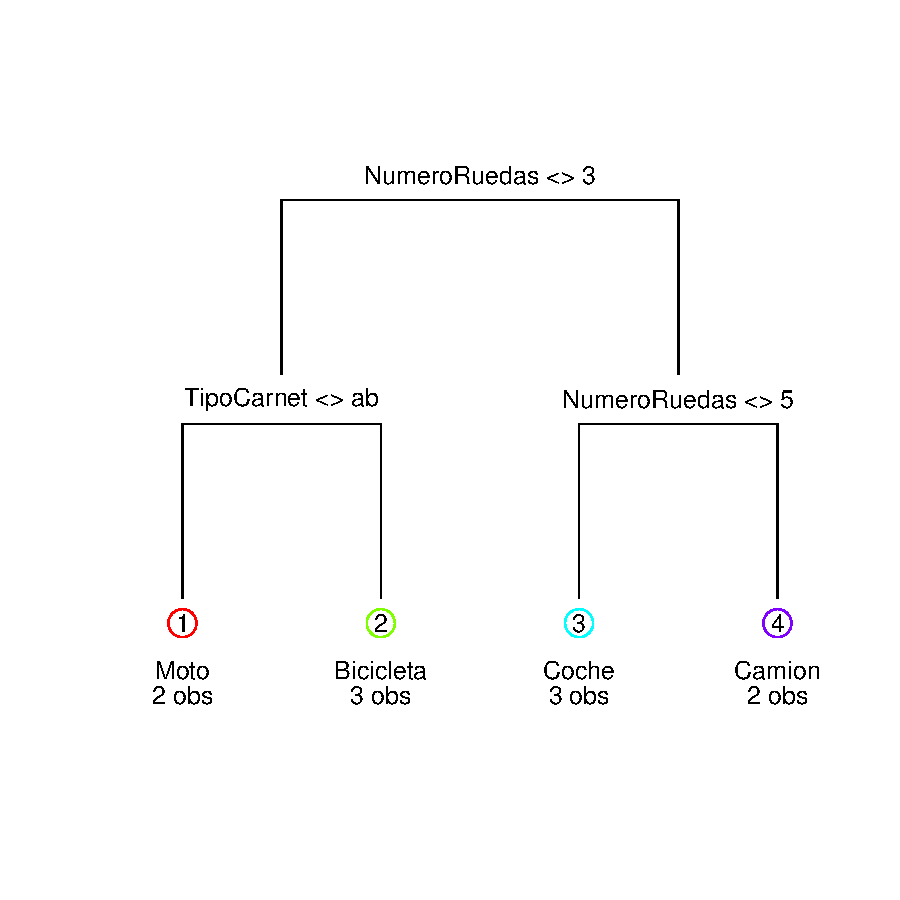
\includegraphics{entrega2-tree_tree}
\end{center}

El arbol generado es igual que el obtenido con rpart con aplicando gini.
Ya que por defecto tree implementa el gini.
En esta libreria no esta implentado el calculo por entropia.



\end{document}
